\chapter{Reguläre Grammatik}

\section{Definition}

\subsection{Definition einer Grammatik}

Eine Grammatik G =(T,N,P,S) besteht aus:

\begin{tabular*}{1.0\textwidth}{l @{\extracolsep{\fill}} l}

T & einer Menge von Terminalsymbolen (kurz Terminalen)\\
N & einer Menge von Nichtterminalsymbolen (kurz Nichtterminale)\\
 & T und N sind disjunkte Mengen\\
 S $\in$ N & einem Startsymbol aus der Menge der Nichtterminale\\
 P $\subseteq$ N $\times$ V* & Menge der Produktionen; (A,x) $\in$ P, A $\in$ N
 und x $\in$ V*; \\
  & statt (A,x) schreibt man A $\rightarrow$ x\\
 V=T $\cup$ N & heißt Vokabular, seine Elemente heißen Symbole\\
 
\end{tabular*}

\subsection{Definition einer rechtslinearen Grammatik}

Eine Grammatik ist regulär, wenn sie entweder eine rechtslineare Grammatik oder
eine linkslineare Grammatik ist.

Eine Grammatik G=G(T,N,P,S) ist einer rechtslineare Grammatik, wenn sie
folgenden Anforderungen genügt:

X $\rightarrow$ a Y \\
X $\rightarrow$ a \\
X $\rightarrow$ $\varepsilon$ \\
mit X,Y $\in$ N und a $\in$ T \\

\section{Datenstruktur}

\subsection{Implementation}

\begin{figure}[h]
  \begin{center}
  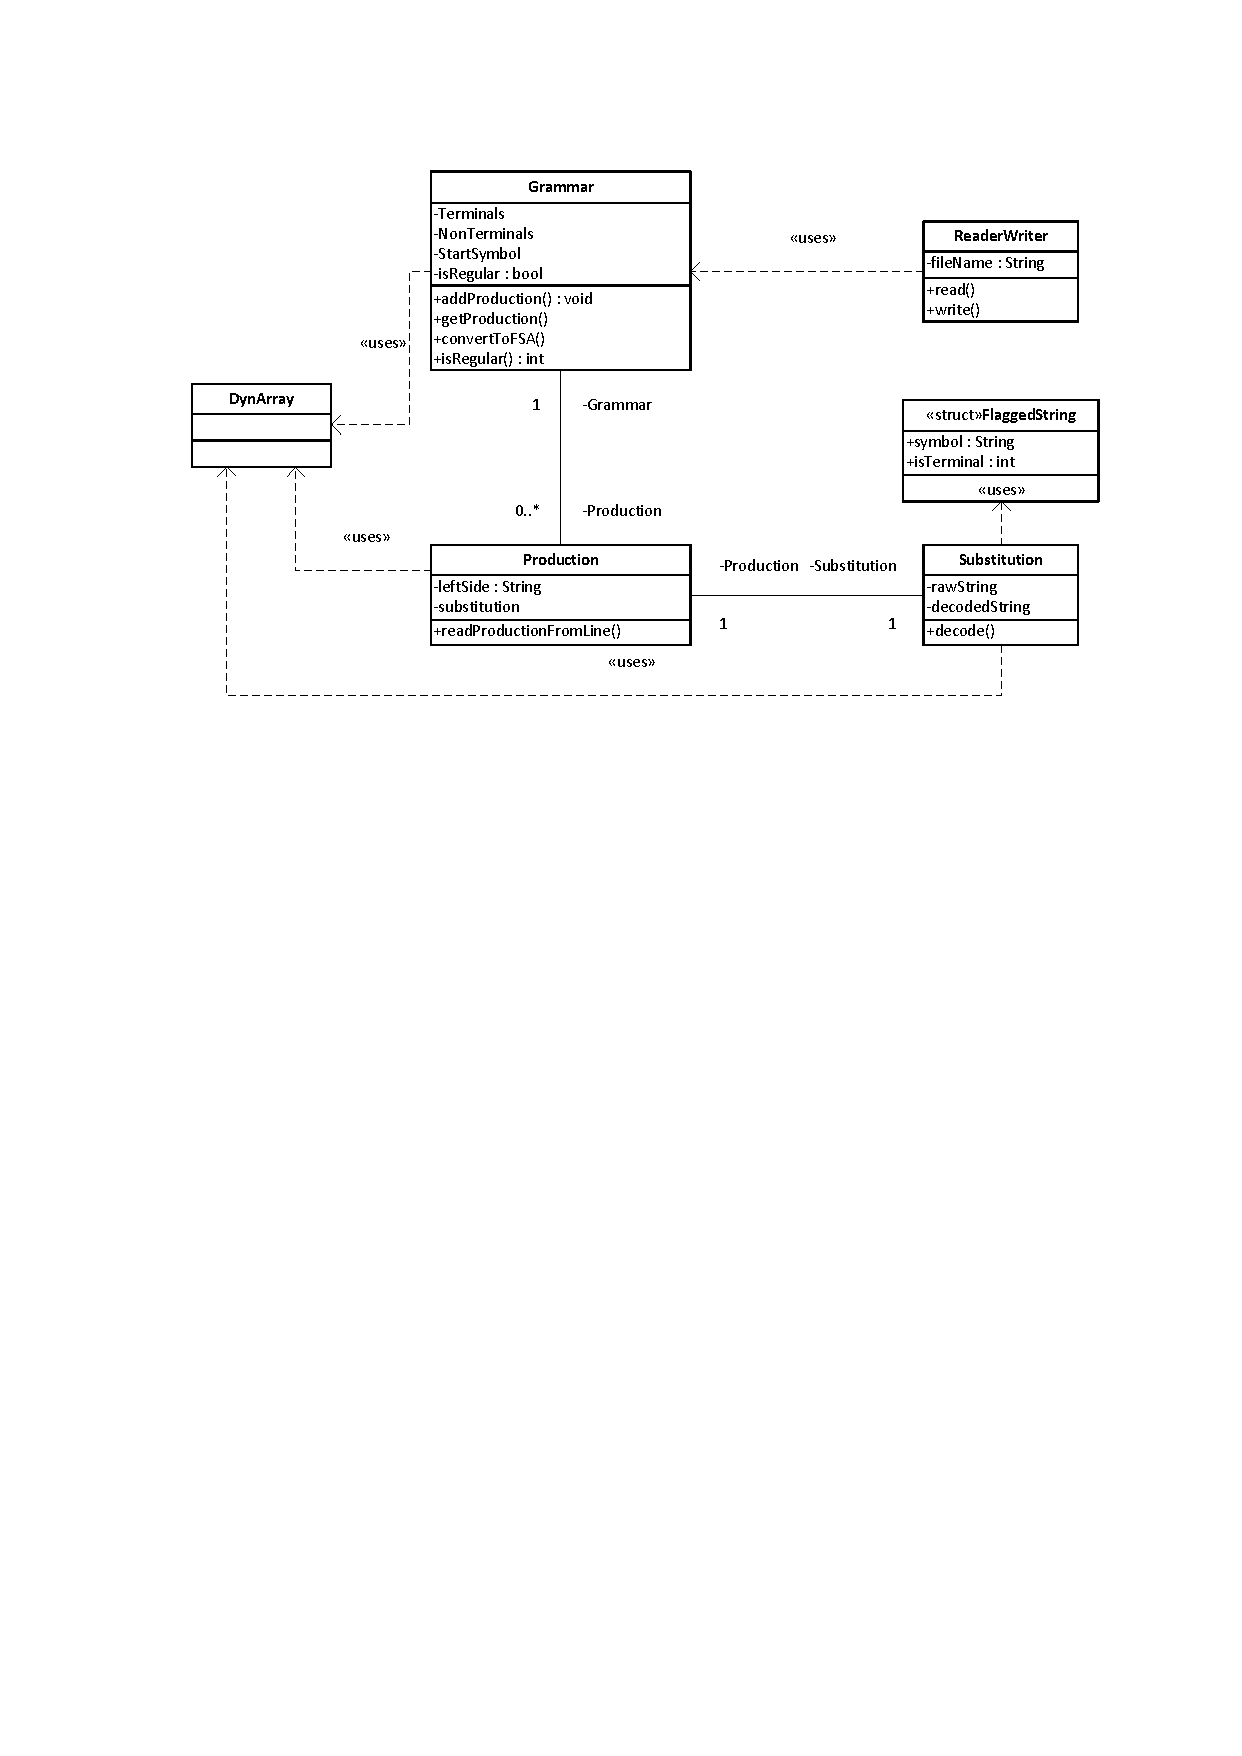
\includegraphics[scale=0.95]{objectsToInclude/UMLGrammar.pdf}
  \caption{Reguläre Grammatik UML Diagramm}
  \label{fig:UMLRegGrammar}
  \end{center}
\end{figure}

Die Klasse \textit{Grammar} besteht aus zwei \textit{dynArrays}
\textit{Terminals} und \textit{NonTerminals}. In diesen werden alle Terminal- und Nichtterminalsymbole
als String gespeichert. Des weiteren besteht ein \textit{Grammar}-Objekt aus
einem String \textit{Startsymbol} für das Startsymbol
der Grammatik, einer Integer Variablen \textit{isRegular}, die angibt ob die Grammatik
regulär ist und einem weitern \textit{dynArray} \textit{Productions} für die
Produktionen. Die Template-Klasse \textit{dynArray} ermöglicht eine unbekannte
Anzahl von Variablen in einem Feld zu speichern, auf die Inhalte des Feldes
wird mit dem [ ]-Operator zugegriffen.

Produktionen bestehen aus einem Nichtterminal auf der linken Seite und einer
Substitution auf der rechten Seite des Pfeils. Die Klasse \textit{Production}
setzt sich aus einer Stringvariablen für die linke Seite und einem Objekt der Klasse
\textit{Substitution} für die rechte Seite zusammen.

Die Klasse \textit{Substitution} enthält eine Zeichenkette \textit{rawString}.
In dieser wird eine unbearbeitete Substitution abgespeichert, also zum Beispiel
direkt nach dem Einlesen, bevor diese dann weiter verarbeitet wird. In einem
\textit{dynArray} vom Typ \textit{flaggedString} wird dann die vollständig
verarbeitete Substitution, unter dem Namen \textit{decodedSubstitution},
gespeichert.

Die Struct \textit{flaggedString} setzt sich aus einem Integer,
der angibt ob das Symbol ein Terminal ist oder nicht, und einem String, der das
Symbol speichert, zusammen. Die Funktion \textit{decode} wandelt nun den
\textit{rawString}, eine Folge von Terminalen und Nichtterminalen, in einen
\textit{flaggedString} Array um, zur Weiterverarbeitung.

\section{Einlesen von regulären Grammatiken}

Es kann mittels der Klasse \textit{RGReaderWriter} eine Grammatik aus einer
Datei eingelesen oder in eine Datei geschrieben werden. Hinter einem Tag folgen die
zugehörigen Symbole. Das Einlesen erfolg zeichenweise.

\lstset{language=C, basicstyle=\footnotesize}
\begin{lstlisting}[float=h!, frame=tb, captionpos=b, caption={Beispiel zu
einem Textdatei der einen Grammatik darstellt.}, label=list:TextGrammar]
[Start]
<expression>
[Terminals]
a
b
c
d
[NonTerminals]
<expression>
[Productions]
<expression> --> a
<expression> --> b <expression>
<expression> --> a b <expression>
<expression> --> c d a b <expression>
<expression> --> d <expression>
\end{lstlisting}
 
\section{Konvertierungen von regulären Grammatiken}

Konvertierungen von einer regulären Grammatik zu einem endlichen Zustandsautomaten
oder einem regulären Ausdruck sind nur möglich, wenn die vorliegende Grammatik
regulär ist. Im Rahmen dieser Projektarbeit wurde eine rechtslinieare Grammatik gewählt.
(Siehe Definition einer rechtslinearen Grammatik).

\subsection{Konvertierung zu einem endlichen Zustandsautomaten}

Eine Transition vom Zustand A zum Zustand B mit a als Eingabe wird in einer
regulären Grammatik als '' A $\rightarrow$ a B `` gespeichert.
Um Zustand B als Endzustand zu setzen gibt es mehrere Möglichkeiten.

1.Fall:

\begin{tabular}{lcr}
B $\rightarrow$ a & $\Longrightarrow$ & B ist ein Endzustand\\
B $\rightarrow$ a B\\
\end{tabular}

Dieser Fall ist aber nicht genau so implementiert: Wird eine Produktion gefunden,
wo die rechte Seite nur ein Terminal ist, dann wird eine neuer Endzustand
erzeugt (leztes Beispiel in Abbildung \ref{fig:convGrammar}). Diese Entscheidung
wurde getroffen, damit nur eine Produktion pro Bearbeitung betrachtet werden
muss. Die zusätzlich erzeugten Zustände werden später entfernt durch die
Konvertierung des Automatens zu einem deterministischen, endlichen
Zustandsautomaten.

2.Fall:

\begin{tabular}{lcr}
B $\rightarrow$ $\varepsilon$ & $\Longrightarrow$ & B ist ein Endzustand\\
\end{tabular}

Ist ein Zustand in einer Transition sowohl Anfang als auch Ende wird dies durch
A $\rightarrow$ a A realisiert: eine Schleife.

\begin{figure}[h]
  \begin{center}
  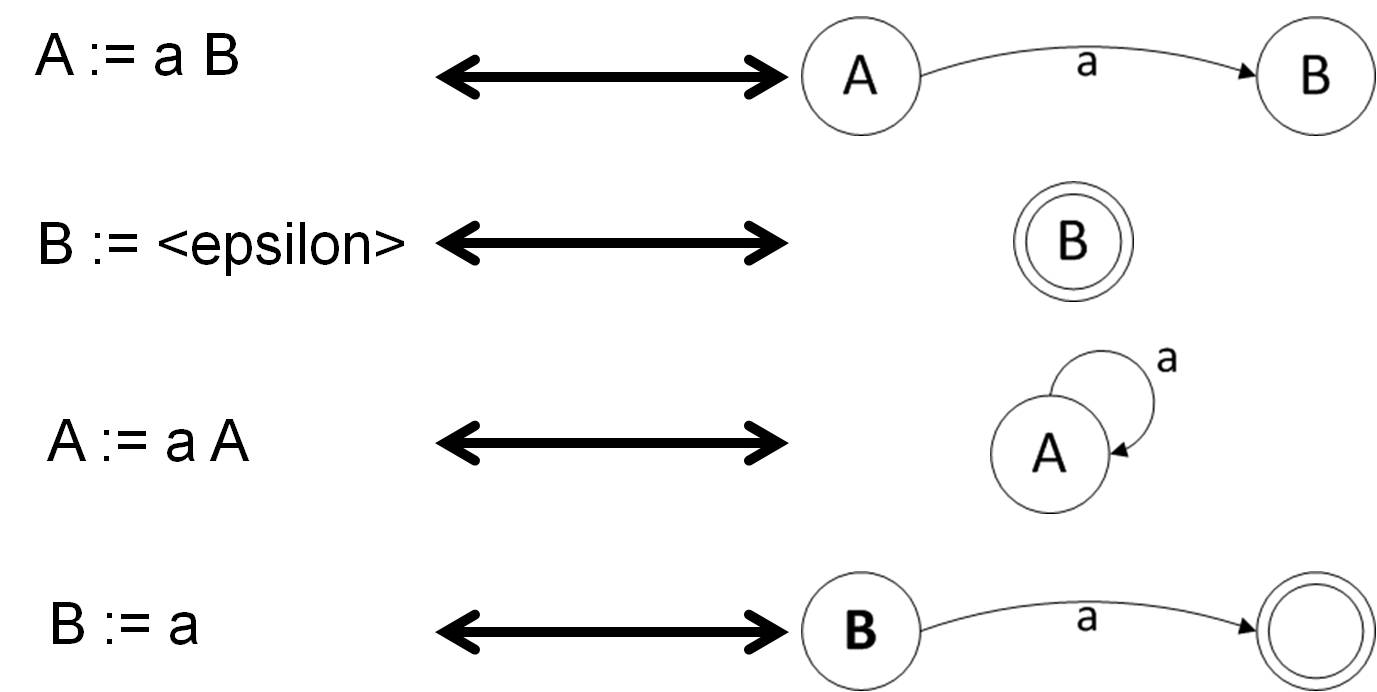
\includegraphics[scale = 0.4]{objectsToInclude/convGram.jpg}
  \caption{Zusammenhang zwischen RG und FSA}
  \label{fig:convGrammar}
  \end{center}
\end{figure}

Für die Umwandlung werden die Produktionen der Reihe nach durchgegangen.
Es gibt 4 mögliche Produktionstypen:

1. A $\rightarrow$ $\varepsilon$ \\
2. A $\rightarrow$ a\\
3. A $\rightarrow$ a A\\
4. A $\rightarrow$ b A , wobei b eine Folge von Terminalen ist.\\

Es wird zuerst überprüft ob die linke Seite im Automaten schon als Zustand
vorhanden ist, falls nicht wird diese dem FSA hinzugefügt. Sollte diese das
Startsymbol sein wird der Zustand als Startzustand gespeichert. Ein Hilfspointer wird
auf diesen Zustand gesetzt.

Ist die rechte Seite das leere Symbol (Fall 1) wird der Zustand als final
markiert und die nächste Produktion umgewandelt, falls nicht wird jedes Symbol
der Substitution durchgegangen.

Ist das aktuelle Symbol ein Terminal und das letzte Symbol der Substitution(Fall 2)
wird ein Zustand Endstate erzeugt und eine Transition vom Hilfpointer zum Endstate
mit dem Terminal als Kante dem Automaten hinzugefügt. Der Endstate wird als
final markiert.

Ist das aktuelle Symbol ein Terminal, nicht das letzte Symbol und wird von einem
Nichtterminal gefolgt (Fall 3), wird das Nichtterminal, falls noch nicht vorhanden,
dem Automaten als Zustand hinzugefügt und eine Transition vom Hilfspointer zum
neuen Zustand mit dem Terminal als Kante erstellt.

Ist das aktuelle Symbol nicht das letzte Symbol, ein Terminal und wird von einem
weiteren Terminal(Fall4 )gefolgt, wird zunächst ein Hilfzustand erzeugt und eine
Transition vom Hilfspointer zum Hilfszustand mit dem Terminal als Kante
hinzugefügt. Der Hilfspointer wird auf den Hilfszustand gesetzt. Dieser Vorgang wird
solange wiederholt bis das aktuelle Symbol ein Terminal und das folgende Symbol ein
Nichtterminal ist. Dann wird, falls noch nicht vorhanden, ein Zustand des
Nichtterminals erzeugt und eine Transition vom Hilfspointer zum neuen Zustand mit
dem Terminal als Kante erstellt. Im Anschluss wird die nächste Produktion
verarbeitet.

\subsection{Konvertierung zu einem regulären Ausdrück}

Eine direkte Konvertierung von einer reguläre Grammatik zu einer regulären
Ausdrück ist im Rahmen dieses Projektes nicht implementiert. Diese Konvertierung
wird aber durch die Konvertierung einer Grammatik zu einem endlichen
Zustandsautomaten und schließlich zu einem regulären Ausdruck realisiert.

Eine direkte Umwandlung ist aber möglich. Die Idee ist im Folgenden dargestellt:
\subsubsection*{Die Grammatik in einer Kompaktform schreiben}
Alle Produktionen mit gleicher linker Seite werden zusammengefasst. z.B:

\begin{tabular}{lcr}

X $\rightarrow$ a Y & & \\
X $\rightarrow$ b Z & $\Longrightarrow$ & X $\rightarrow$ a Y | b Z
|$\varepsilon$\\
X $\rightarrow$ a $\varepsilon$ & &\\
 
\end{tabular}

\subsubsection*{Die Produktionen als gleichungen interpretieren}

Dafür werden die $\rightarrow$ zu ``=``  und die ``|'' zu ``+'' umgewandelt.
z.B:

\begin{tabular}{lcr}

X $\rightarrow$ a Y | b Z |$\varepsilon$ & $\Longrightarrow$ & X = a Y + b Z
+$\varepsilon$\\

 
\end{tabular}

\subsubsection*{Das Gleichungssystem lösen}

Gesucht ist eine Gleichung die nur das Startsymbol als Variable enthält.

Die Distributivität und Assoziativität sind hier zwei verwendbare Eigenschaften der
gewöhlichen ``+'' Operation. Zusätzlich, können Produktionen der Form A = c A +
B in die Form A = c* B umgewandelt werden.
